%!TEX ROOT=main.tex

\section{Module design}
As discussed in section \ref{section:module-architecture}, where the LoRa module was architected and its main parts were selected, the schematic and board layout were created. These outputs are included in image form as Appendix \ref{chapter:module01-files} along with more details and available at (https://github.com/manakjiri/lora-module-hw/releases/tag/v0.1)?.

The Open source KiCad Electronic Design Automation software was used throughout the project to create these designs. 

\subsection{Schematic}
While the \ref{section:module-architecture} focused on the fundamental parts of the design, many details were left up to the later development stages, once the overall system implementation is more clear. This section will focus and expand on these parts of the design.

Of note is the selection of the main clock source for the MCU \ref{section:mcu}. In this case the only two options are to use a Crystal oscillator (XO) or an Temperature Compensated XO (TCXO). Application note AN5646 (STMicroelectronics) summarizes the main differences as
\begin{itemize}
    \item An XO is more efficient on power consumption, startup time, and BOM cost.
    \item A TCXO is more efficient on frequency accuracy and frequency variation over temperature changes. It also
    removes layout constraints.
\end{itemize}

This aspect was not considered carefully enough during the parts selection, the recommended NX2016SA series crystal oscillator was selected for the power savings and reduced cost. The selected programming framework embassy, and lora-rs in particular (expanded upon in Appendix \ref{chapter:rust}), only correctly supported the use of an TCXO, at the time of the prototype bring-up. This led to an ad-hoc modification of the module and the addition of the Abracon ATX-11-F series TCXO to fix this issue.

All other aspects of the MCU integration were executed according to the application notes (cite), the datasheet and closely followed the implementations of the reference design and the nucleo development kit. This includes the selection of decoupling capacitors, the SMPS circuitry and the reset handling.

Another consideration was the implementation of the switchable power rail VDD\_SW. This rail taps off the main power rail of the rest of the module, any disruption could cause a glitch or trigger the BOR protection circuitry. It is thus necessary to limit the inrush current caused by this rail's switch-on and subsequent charging of any local capacitances.

dopsat vypocty casu

\subsection{Board layout}
A 4 layer board stackup was proposed in Section \ref{section:mcu}, which indeed ended up being used in this design. Purpose of each layer is described in table \ref{table:board-layers} and clearly observable in the final renders \ref{board:v0.1}.

\begin{table}[H]
\begin{center}
\caption{\label{table:board-layers}Module board layer signal and power assignments}
    \begin{tabular}{|l|l|} \hline
    \textbf{Layer name}     & \textbf{Primary purpose} \\ \hline
    F. Front layer          & Components and local connections \\ \hline
    1. First inner layer    & Ground \\ \hline
    2. Second inner layer   & Power \\ \hline
    B. Back layer           & Signal and markings \\ \hline
    \end{tabular}
\end{center}
\end{table}

The board is only populated on the front side \ref{board:v0.1-components}, to allow its use as a solder-able module. Still, the final dimensions of the module are $20.32 \times 22.48~\mathrm{mm}$, which is better than the initial optimistic estimate given in \ref{section:antenna}.

To stay compatible with low-cost manufacturing options, conservative parameters were picked when it comes to minimal clearance, trace width and drill size. No density-increasing technologies, such as blind or buried vias, via-in-pad, micro-via, etc. were not employed either. 

These parameters are summarized in the following Table \ref{table:board-limits} and were enforced by the Design Rule Checker (DRC) throughout the project.

\begin{table}[H]
\begin{center}
\caption{\label{table:board-limits}Board layout physical limits}
    \begin{tabular}{|l|l|} \hline
    \textbf{Parameter}          & \textbf{Dimension} \\ \hline
    Minimum trace clearance & $0.150~\mathrm{mm}$ \\ \hline
    Minimum trace width & $0.150~\mathrm{mm}$ \\ \hline
    Minimum via width & $0.300~\mathrm{mm}$ \\ \hline
    Hole to trace clearance & $0.254~\mathrm{mm}$ \\ \hline
    Hole to hole clearance & $0.500~\mathrm{mm}$ \\ \hline
    Board edge to trace clearance & $0.150~\mathrm{mm}$ \\ \hline
    \end{tabular}
\end{center}
\end{table}

Being only 4 layers, the traces needed to be routed in densely and well thought-out manner, attempting to minimize the number of relatively large vias required. For this reason, the module's external connection signal assignments were decided only near the end of the design stage conforming mostly to the existing pin locations on the MCU itself. The final pad assignments are included in Table \ref{table:module-pin-legend}.

\subsection{Final module specification}
\begin{figure}
    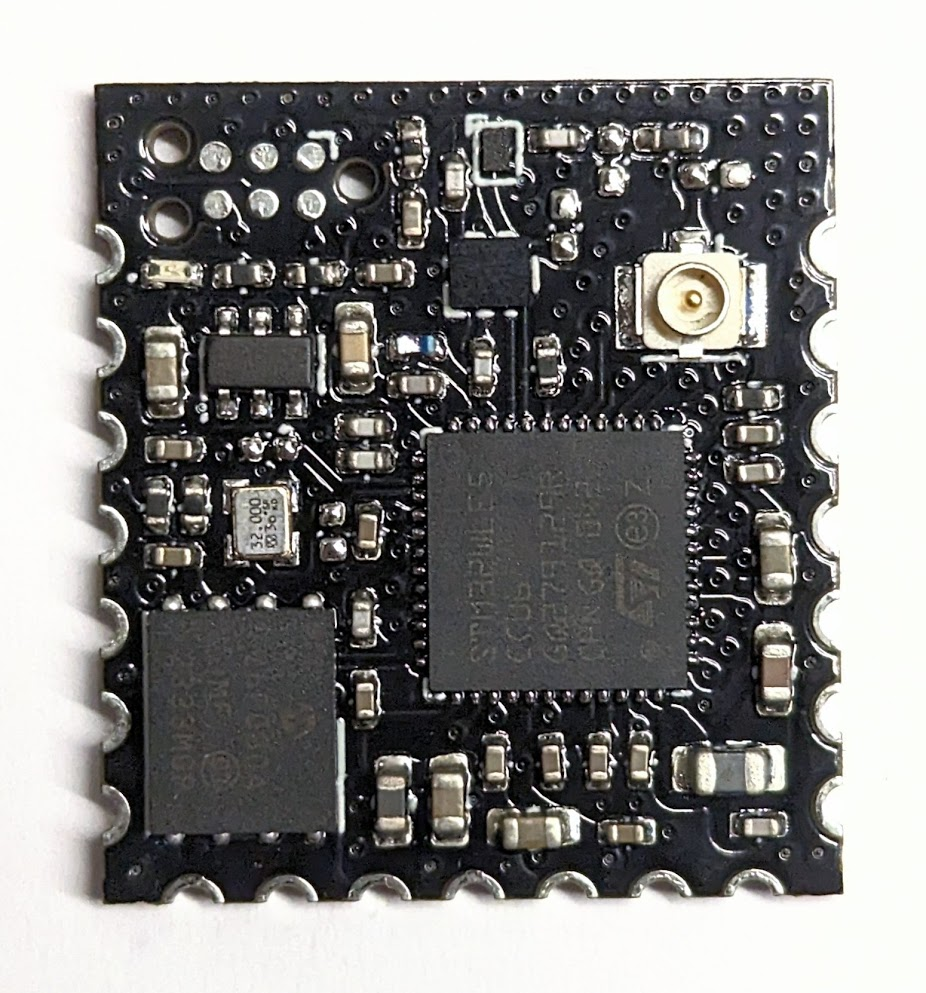
\includegraphics[width=.45\textwidth]{img/module-v0.1.jpg}
    \caption{\label{fig:module-v0.1}Image of the manufactured and fully assembled module}
\end{figure}

\begin{table}[H]
\begin{center}
\caption{\label{table:module-specification}Final module specification}
    \begin{tabular}{|l|l|} \hline
    Supply voltage range                    & $2.3\text{--}3.5~\mathrm{V}$\\ \hline
    Maximum supply current (excluding EXT)  & $65~\mathrm{mA}$\\ \hline
    Standby supply current                  & $?~\mathrm{uA}$\\ \hline
    Operating temperature range             & $-40\text{--}85~\mathrm{^\circ C}$\\ \hline
    Output RF power                         & $15~\mathrm{dB}$\\ \hline
    Operating band                          & $868~\mathrm{MHz}$\\ \hline
    RF connector                            & U.FL \\ \hline
    Module connection type                  & Castellated hole (0.1 inch pitch) \\ \hline
    Supported interfaces                    & UART, SPI, I2C \\ \hline
    Programming interface                   & ARM Serial Wire Debug \\ \hline
    \end{tabular}
\end{center}
\end{table}

\begin{table}[H]
\begin{center}
\caption{\label{table:module-pin-legend}Module pin legend including feature summary. Refer to each column following ``Pin'' (excluding ``Other'') as [Column header][Column-row contents], such as ``SPI1\_MOSI'' and so on. Some features were omitted for clarity, for complete list refer to the MCU manufacturer's documentation}
    \begin{tabular}{|l|l|l|l|l|l|l|l|l|} \hline
    \textbf{Name} & \textbf{Pin} & \textbf{TIM} & \textbf{ADC} & \textbf{I2C} & \textbf{SPI} & \textbf{UART} & \textbf{Other}\\ \hline
    1        & PA7  & 17\_1, 1\_1N    &     & 3\_SCL & 1\_MOSI &             & CMP2\_OUT          \\ \hline
    2        & PA6  & 16\_1          &     &       & 1\_MISO &             &                    \\ \hline
    3        & PA4  & L1,2\_OUT      &     &       &        &             & RTC\_OUT2           \\ \hline
    4        & PA2  & 2\_3           &     &       &        & 2\_TX & CMP2\_OUT           \\ \hline
    5        & PA1  & L3\_OUT, 2\_2   &     &       & 1\_SCK  &             &                    \\ \hline
    6        & PA0  & 2\_1           &     &       &        &             & WKUP1   \\ \hline
    7        & PB8  & 16\_1, 1\_2N    &     & 1\_SCL &        &             &                    \\ \hline
    8        & PB7  & L1\_IN2, 17\_1N &     & 1\_SDA &        & 1\_RX        &                    \\ \hline
    9        & PB6  &               &     & 1\_SCL &        & 1\_TX        &                    \\ \hline
    10       & PB5  & L1\_IN1        &     &       & 1\_MOSI &             & CMP2\_OUT          \\ \hline
    11       & PB4  &               & 3   & 3\_SDA & 1\_MISO &             & CMP1,2\_INP        \\ \hline
    12       & PA11 & 1\_4           & 7   & 2\_SDA & 1\_MISO &             & CMP1,2\_INM        \\ \hline
    SWO/13   & PB3  & 2\_CH2         & 2   &       & 1\_SCK  &             & WKUP3 \\ \hline
    SWDIO/14 & PA13 &               & 9   &       &        &             & IR\_OUT             \\ \hline
    SWCLK/15 & PA14 & L1\_OUT        & 10  &       &        &             &                    \\ \hline
    BOOT0/16 & PH3  &               &     &       &        &             &                    \\ \hline
    \end{tabular}
\end{center}
\end{table}
